\documentclass[tikz=true]{standalone}
\usepackage{graphicx, standalone}
\usepackage[compat=1.1.0]{tikz-feynman}
\usepackage{tikz}
\usepackage{amsmath, amssymb}
\usepackage{euler}
\usepackage{fontspec}
\setmainfont{MinionPro}

\begin{document}

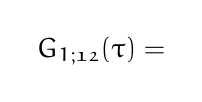
\begin{tikzpicture}[baseline=(current bounding box.center)]
    \node {$G_{1;\mathfrak{12}}(\tau)=$};
\end{tikzpicture}
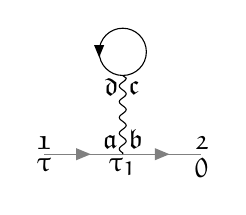
\begin{tikzpicture}[baseline=(current bounding box.base)]
	\begin{feynman}[small]
		\vertex (a);
		\vertex[right=of a] (b);
		\vertex[right=of b] (c);
		\vertex[above=of b] (b1);
		
		\node[above=-0.2em of a] {$\mathfrak{1}$};
		\node[above left=-0.2em of b] {$\mathfrak{a}$};
		\node[above right=-0.2em of b] {$\mathfrak{b}$};
		\node[above=-0.2em of c] {$\mathfrak{2}$};
		\node[below left=-0.25em and -0.2em of b1] {$\mathfrak{d}$};
		\node[below right=-0.2em of b1] {$\mathfrak{c}$};
		
		\node[below=-0.2em of a] {$\tau$};
		\node[below=-0.2em of b] {$\tau_1$};
		\node[below=-0.2em of c] {$0$};
		
		\def\r{0.3}
		
		\path (b1)--++(90:\r) coordinate (A);
		\draw[fermion, arrow size=1pt] (A) circle(\r);		
		
		\diagram* {
			(a) -- [fermion, gray] (b) -- [fermion, gray] (c),
			(b) -- [photon] (b1)
		};	
	\end{feynman}
\end{tikzpicture}
\begin{tikzpicture}[baseline=(current bounding box.center)]
    \node {$+$};
\end{tikzpicture}
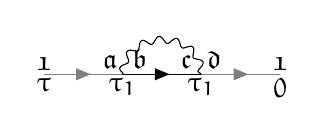
\begin{tikzpicture}[baseline=(current bounding box.base)]
	\begin{feynman}[small]
		\vertex (a);
		\vertex[right=of a] (b);
		\vertex[right=of b] (c);
		\vertex[right=of c] (d);
		
		\node[above=-0.2em of a] {$\mathfrak{1}$};
		\node[above left=-0.2em of b] {$\mathfrak{a}$};
		\node[above right=-0.15em and -0em of b] {$\mathfrak{b}$};
		\node[above left=-0.15em and -0em of c] {$\mathfrak{c}$};
		\node[above right=-0.2em of c] {$\mathfrak{d}$};
		\node[above=-0.2em of d] {$\mathfrak{1}$};
		
		\node[below=-0.2em of a] {$\tau$};
		\node[below=-0.2em of b] {$\tau_1$};
		\node[below=-0.2em of c] {$\tau_1$};
		\node[below=-0.2em of d] {$0$};
		
		\diagram* {
			(a) -- [fermion, gray] (b),
			(b) -- [fermion] (c),
			(c) -- [fermion, gray] (d),
			(b) -- [photon, half left] (c)
		};
	\end{feynman}
\end{tikzpicture}

\end{document}